\documentclass[10pt]{beamer}
\usetheme{metropolis}  
\usecolortheme{beaver}
\usepackage{hyperref}
\usepackage{bigints}
\usepackage{amsmath}

\title{Introducci\'on a la probabilidad y estad\'istica CM274}
 \usepackage[spanish]{babel}
 \decimalpoint
\date{\today}
\author{C\'esar Lara Avila}
\institute{\url{https://github.com/C-Lara}}
\begin{document}
  \maketitle
  \section{6. Variables aleatorias continuas }
  
\begin{frame}{Introducci\'on}

\small {Todas las variables aleatorias asignan un n\'umero a cada resultado en un espacio muestral. Mientras que las variables aleatorias discretas asumen un conjunto discreto de valores posibles, las variables aleatorias continuas tienen un conjunto continuo de valores.}
	

\vspace{0.6cm}


\scriptsize{\textcolor{blue}{\textbf {Ejemplo 1}}  Dado que el tiempo es continuo, la cantidad de tiempo que Luis por llegar  temprano (o tarde) para la clase es una variable aleatoria continua. 

Supongamos que 	se mide cu\'anto Luis llega temprano a la clase cada dia (en unidades de minutos). Es decir, el resultado de un ensayo en nuestro experimento es un tiempo en minutos. Asumiremos que hay fluctuaciones aleatorias en el momento exacto en que aparece. Dado que en principio Luis pod\'ia llegar, por ejemplo, a $3.43$ minutos de anticipaci\'on, o $2.7$ minutos de retraso (correspondiente al resultado $-2,7$), o en cualquier otro momento, el espacio muestral consta de todos los n\'umeros reales.

As\'i, la variable aleatoria que da el resultado en s\'i tiene un \textcolor{blue}{rango continuo de valores posibles}. 
	
}
\end{frame}

\begin{frame}{C\'alculo}
\small {Aunque asumiremos que tu puedes calcular las formas m\'as familiares de derivados e integrales a mano. Pero las expresiones delicadas, dejaremos que la computadora haga la mayor parte del c\'alculo. 
	
Conceptualmente, debes estar confortable  con dos puntos de vista de una integral definida.

\begin{enumerate}
	\item $\bigints_{a}^{b}f(x) dx = \text{area bajo la curva}\ y = f(x).$
	\item $\bigints_{a}^{b}f(x) dx = \text{suma de}\ f(x) dx.$
\end{enumerate}

\vspace{0.2cm}

La conexi\'on entre los dos puntos de vista:

\begin{align*}
\text{\'area } \approx \text{suma de \'area rect\'angulos} &= f(x_1)\Delta x + f(x_2)\Delta x + \dots f(x_n)\Delta x \\ & = \sum_{1}^{n}f(x_i)\Delta x.
\end{align*}
}
\end{frame}

\begin{frame}{C\'alculo}
\small{ 

A medida que la anchura $\Delta x$ de los intervalos se hace m\'as peque\~na, la aproximaci\'on se hace mejor.

\begin{figure}[ht]
	\centering
	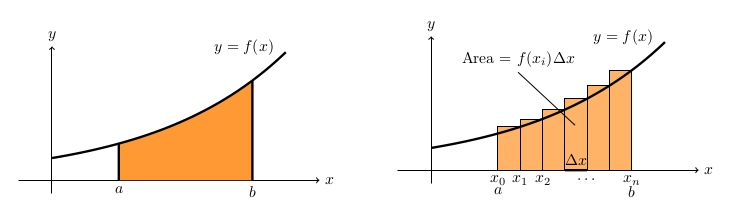
\includegraphics[scale=.4]{G1.png}
\end{figure}
	}
	

\vspace{0.4cm}

\scriptsize{En el c\'alculo aprendiste a calcular integrales encontrando antiderivadas. Esto es importante para los c\'alculos, pero no confundas este m\'etodo con la raz\'on por la que usamos integrales.
	
Nuestro inter\'es en las integrales proviene principalmente de su interpretaci\'on como una \texttt{suma} y en mucho menor grado su interpretaci\'on como \'area.}	
\end{frame}

\begin{frame}{Variables aleatorias continuas }
\small{ Una variable aleatoria continua toma un rango de valores, que puede ser finito o infinito en extensi\'on. Aqu\'i hay algunos ejemplos de rangos: $[0, 1]$, $[0, \infty)$, $(-\infty, \infty)$, $[a, b]$.

\textcolor{green}{\textbf{Definici\'on:}} Una variable aleatoria $X$ es \textcolor{violet}{continua}, si existe una funci\'on continua $f(x)$ tal que para alg\'un $c \leq d$, tenemos

\begin{equation}
\mathbb{P}(c \leq X \leq d) = \bigintsss_{c}^{d}f(x)dx
\end{equation}

La funci\'on $f(x)$ es llamada la \textcolor{blue}{\textbf{funci\'on de densidad de probabilidad} (PDF)}. El PDF satisface las siguientes propiedades:

\begin{enumerate}
	\item $f(x) \geq 0$ (f es no negativa).
	\item $\bigintsss_{-\infty}^{\infty}f(x)dx = 1$ \quad (esto es equivalente a: $\mathbb{P}(-\infty < X <  \infty) = 1)$.
\end{enumerate}
	}
\end{frame}

\begin{frame}{Funci\'on de  densidad de probabilidad }
\small{ La funci\'on de densidad de probabilidad $f(x)$ de una variable aleatoria continua es el an\'alogo de la funci\'on de masa de probabilidad $p(x)$ de una variable aleatoria discreta. Aqu\'i hay dos diferencias importantes:

\begin{enumerate}	
	
\item A diferencia de $p(x)$, el PDF $f(x)$ no es una probabilidad. Tienes que integrar  para obtener la  probabilidad. 
\item Como $f(x)$ no es una probabilidad, no hay restricci\'on de que $f(x)$ sea menor o igual a $1$.
\end{enumerate}

\textcolor{red}{\textbf{Notas:}}

En la propiedad 2, hemos integrado sobre $(-\infty, \infty)$ ya que no conoc\'iamos el rango de valores tomado por $X$. Formalmente, esto tiene sentido porque simplemente definimos $f(x)$ como $0$ fuera del rango de $X$. 

En la  pr\'actica, debemos integrar entre los l\'imites dados por el rango de $X$.
}		
\end{frame}

\begin{frame}{Vista gr\'afica de la probabilidad }
\small{ Si se grafica la funci\'on de densidad de probabilidad de una variable aleatoria continua $X$ entonces
	
\[
\mathbb{P}(c \leq X \leq d) = \text{\'area bajo la gr\'afica entre c y d}.
\]

\begin{figure}[ht]
	\centering
	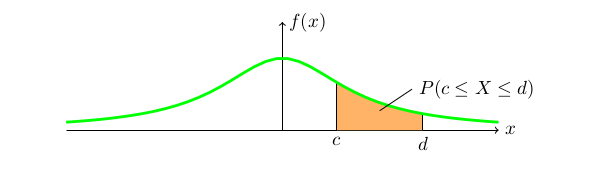
\includegraphics[scale=.4]{G2.png}
\end{figure}

\textcolor{yellow}{\textbf{Pregunta:}}

?`Cu\'al es el \'area total bajo el PDF $f(x)$?.
}

\end{frame}

\begin{frame}{Los t\'erminos: masa de probabilidad y densidad de probabilidad}
\small{ ?`Por qu\'e usamos los t\'erminos masa y densidad para describir el PMF y el PDF? ?`Cu\'al es la diferencia entre los dos? 

La respuesta simple es que estos t\'erminos son completamente an\'alogos a la masa y la densidad que se vi\'o en la f\'isica y el c\'alculo. Vamos a revisar esto primero para la funci\'on de masa de probabilidad y luego discutir la funci\'on de densidad de probabilidad.

\textcolor{green}{\textbf{Masa con una suma:}}

Si las masas $m_1, m_2, m_3$ y $m_4$ son puestas en las posiciones $x_1, x_2, x_3$ y $x_4$, entonces la masa de probabilidad es  $m_1 + m_2 + m_3 + m_4.$

\begin{figure}[ht]
	\centering
	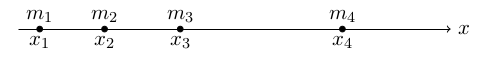
\includegraphics[scale=.4]{G3.png}
\end{figure}

Podemos definir una funci\'on de masa $p(x)$ con $p(x_j) = m_j$ para $j = 1, 2, 3, 4$, y $p(x) = 0$ en caso contrario. 
}
\end{frame}

\begin{frame}{Los t\'erminos: masa de probabilidad y densidad de probabilidad}
\small{En esta notaci\'on la masa total es $p(x_1) + p(x_2) + p(x_3) + p (x_4)$.
	
La \textcolor{blue}{funci\'on de masa de probabilidad} se comporta exactamente de la misma manera, excepto que tiene la dimensi\'on de probabilidad en lugar de masa.

\textcolor{green}{\textbf{Masa con una integral de densidad:}}

Supongamos que se tiene una varilla de longitud $L$ metros con densidad variable $f(x)kg/m$. (Observa que las unidades son de masa/longitud.)

\begin{figure}[ht]
	\centering
	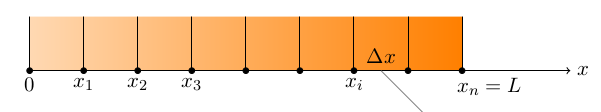
\includegraphics[scale=.4]{G4.png}
	\hspace{6.5cm} $\text{masa de la i-\'esima pieza} \approx f(x_i)\Delta x$
\end{figure}
}

\end{frame}

\begin{frame}{Los t\'erminos: masa de probabilidad y densidad de probabilidad}
\small{ Si la densidad var\'ia continuamente, debemos encontrar la masa total de la barra por integraci\'on:
	
\[
\text{masa total} = \bigintsss_{0}^{L}f(x)dx.
\]

Esta f\'ormula viene de dividir la barra en peque\~nas piezas y sumando  la masa de cada pieza. Es decir:

\[
\text{masa total} \approx \sum_{i =1}^{n}f(x_i)\Delta x
\]


En el l\'imite cuando $\Delta x$ tiende  a cero, la suma se convierte en integral.

La \textcolor{orange}{funci\'on de densidad de probabilidad} se comporta exactamente de la misma manera, excepto que tiene unidades de probabilidad/(unidad $x$) en lugar de $kg/ m$. De hecho, la ecuaci\'on (1) es exactamente an\'aloga a la integral anterior para la masa total.
		
}
\end{frame}

\begin{frame}{Ejemplo}
\small{
\textcolor{blue}{\textbf {Ejemplo 2}} Supongamos que $X$ tiene un pdf $f(x) = 0$ en $[0, 1/3]$ (esto significa que $f(x) = 0$ fuera de $[0, 1/3]$). Grafiquemos el pdf y calculemos $\mathbb{P}(.1 \leq X \leq .2)$ y $\mathbb{P}(.1 \leq X \leq 1)$. 

En efecto:  $\mathbb{P}(.1 \leq X \leq .2)$, es mostrado a la izquierda de la figura que continua. Calculemos la integral:

\[
\mathbb{P}(.1 \leq X \leq .2) = \int_{.1}^{.2}f(x) dx = \int_{.1}^{.2}3dx = .3
\]

O podemos encontrar el \'area geom\'etricamente:

\[
\text{\'area del rect\'angulo} = 3 \cdot .1 = .3
\]

$\mathbb{P}(.1 \leq  X \leq  1)$ se muestra a la derecha de la figura que continua. Puesto que hay un \'area bajo $f(x)$ hasta $1/3$, tenemos $\mathbb{P}(.1 \leq X \leq 1) = 3 \cdot (1/3 - .1) = .7$.
}
\end{frame}

\begin{frame}{Ejemplo}
	\small{
\begin{figure}[ht]
	\centering
	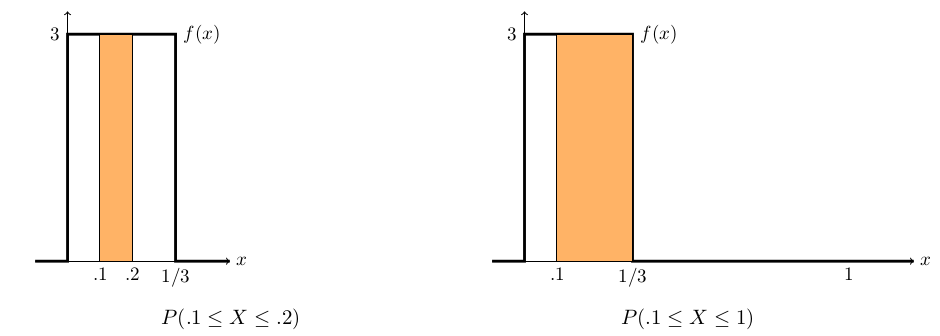
\includegraphics[scale=.27]{G5.png}
	
\end{figure}

\textcolor{blue}{\textbf{Preguntas:}}

\begin{enumerate}
\item En el ejemplo anterior $f(x)$ toma valores mayores que $1$. ?`Por qu\'e esto no viola la regla de que las probabilidades est\'an siempre entre $0$ y $1$?.

\item Sea $X$ una variable aleatoria continua:

\begin{itemize}
	\item ?` Qu\'e es $\mathbb{P}(a \leq X \leq a)$?
	\item ?` Qu\'e es $\mathbb{P}(X = 0)$?
	\item ?` $\mathbb{P}(X = a) = 0$ significa que $X$ no puede ser igual $a$?
\end{itemize}
\end{enumerate}
}

\end{frame}

\begin{frame}{Notaci\'on}
\small{ Podemos definir una variable aleatoria dando su rango y una funci\'on de densidad de probabilidad.

\vspace{0.2cm}
		
Por ejemplo podr\'iamos decir, sea $X$ una variable aleatoria con rango $[0,1]$ y pdf $f(x) = x/2$. Impl\'icitamente, esto significa que $X$ no tiene densidad de probabilidad fuera del rango dado. Si quisi\'eramos ser absolutamente rigurosos, dir\'iamos expl\'icitamente que $f(x) = 0$ fuera de [0,1], pero en la pr\'actica esto no ser\'a necesario.
}

\vspace{2.8cm}


\end{frame}

\begin{frame}{Funci\'on de distribuci\'on acumulativa}
\small{La funci\'on de distribuci\'on acumulativa CDF de una variable aleatoria continua $X$ es definida de igual manera que el CDF de las variables aleatorias discretas.

\[
F(b) = \mathbb{P}(X \leq b).
\]

\vspace{0.3cm}

Ten en cuenta que la definici\'on es acerca de la probabilidad. Al usar el cdf primero debes pensar en que es una probabilidad. Entonces cuando lo vaa a calcular, puedes utilizar,

\[
F(b) = \mathbb{P}(X \leq b) = \int_{-\infty}^{b}f(x) dx, \quad \text{donde }\  f(x)\  \text{es el pdf  de X }.
\]	
}
\end{frame}
\begin{frame}{Algunas observaciones}
\small{ \textcolor{violet}{\textbf{Notas:}}
		
\begin{enumerate}
\item Para las variables aleatorias discretas, hemos definido la funci\'on de distribuci\'on acumulativa, pero no tuvimos mucha ocasi\'on de usarlo. El cdf desempe\~na un papel mucho m\'as prominente para las variables aleatorias continuas.
	
\item Como antes, iniciamos la integral en $-\infty$ porque no conoc\'iamos el rango preciso de $X$. Formalmente, esto todav\'ia tiene sentido ya que $f(x) = 0$ fuera del rango de $X$. En la pr\'actica, conoceremos el rango y inicializaremos la integral al inicio del rango.

\item En la pr\'actica, a menudo decimos \textcolor{yellow}{$X$ tiene distribuci\'on F (x)} en lugar de $X$ tiene funci\'on de distribuci\'on acumulativa $F(x)$.
\end{enumerate}

}
\end{frame}
\begin{frame}{Ejemplo}
\small{\textcolor{blue}{\textbf {Ejemplo 3}} Encontremos el cdf, para el pdf $f(x) = 3x^2$ en $[0,1]$. Supongamos $X$ es una variable con esa distribuci\'on. Hallemos tambi\'en  $\mathbb{P}(X < 1/2)$.

\vspace{0.2cm}

$f(x) = 3x^2 en \  [0,1] \rightarrow F(a) = \int_{0}^{a}3x^2 dx = a^3\ \text{en}\ [0,1]$. Por tanto:

\[
F(a) = \begin{cases}
0 & \text{si}\  a <  0 \\
a^3 & \text{si}\  0 \leq a \leq 1 \\
1 & \text{si}\  1 < a
\end{cases}
\]

\vspace{0.2cm}

Aqu\'i los gr\'aficos de $F(x)$ y $f(x)$, as\'i como el valor pedido $\mathbb{P}(X < 1/2) = F(1/2) = 1/8$.


\begin{figure}[ht]
	\centering
	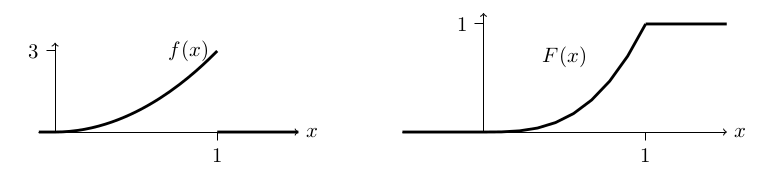
\includegraphics[scale=.35]{G6.png}
\end{figure}


}
\end{frame}

\begin{frame}{Propiedades de la funci\'on de distribuci\'on acumulativa}
\small{A continuaci\'on se presenta un resumen de las propiedades m\'as importantes de la funci\'on de distribuci\'on acumulativa (CDF)

\begin{enumerate}
\item (Definici\'on) $F(x) = \mathbb{P}(X \leq x)$
\item $0 \leq F(x) \leq 1$
\item $F(x)$ es no decreciente, esto es, si $a \leq b$ entonces $F(a) \leq F(b)$.
\item $\lim_{x \rightarrow \infty} F(x) =1$ y  $\lim_{x \rightarrow -\infty} F(x) =0$
\item $\mathbb{P}(a \leq X \leq b) = F(b) -F(a)$
\item (Teorema fundamental del c\'alculo) $F^{'}(x) = f(x)$.
\end{enumerate}

Las propiedades $2$, $3$, $4$ son id\'enticas a las de las distribuciones discretas.
	
}
\end{frame}
\begin{frame}{Propiedades de la funci\'on de distribuci\'on acumulativa}
\small{ La propiedad 5, puede ser vista algebraicamente:
	
\begin{align*}
\int_{-\infty}^{b}f(x) dx &= \int_{-\infty}^{b}f(x) dx +  \int_{-\infty}^{b}f(x) dx \\
\Leftrightarrow \int_{-\infty}^{b}f(x) dx &=  \int_{-\infty}^{b}f(x) dx +  \int_{-\infty}^{b}f(x) dx \\
\Leftrightarrow \mathbb{P}(a \leq X \leq b) &= F(b) - F(a).
\end{align*}

\vspace{0.2cm}

La propiedad 5 tambi\'en puede verse geom\'etricamente. La regi\'on anaranjada representa $F(b)$ y la regi\'on de rayas representa $F(a)$. Su diferencia es $\mathbb{P}(a \leq  X \leq b)$.

\begin{figure}[ht]
	\centering
	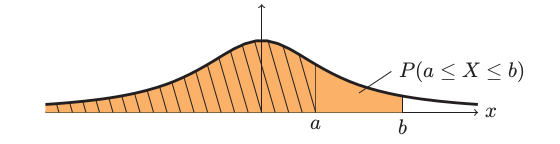
\includegraphics[scale=.4]{G7.png}
\end{figure}
}
\end{frame}

\end{document}